\documentclass[12pt,letterpaper]{article}
% \documentclass[journal=acsomega,manuscript=article]{achemso}
\usepackage{fullpage}
\usepackage[top=1.5cm, bottom=3.5cm, left=2.2cm, right=2.2cm]{geometry}
\usepackage{amsmath,amsthm,amsfonts,amssymb,amscd, esint}
\usepackage{lastpage}
\usepackage{enumerate}
\usepackage{fancyhdr}
\usepackage{mathrsfs}
\usepackage{graphicx}
\usepackage{listings}
\usepackage{hyperref}
\usepackage[english]{babel}
\usepackage{lipsum}
\usepackage[table,xcdraw]{xcolor}
\usepackage{enumitem}
\usepackage{pgfplots}
\usepackage{float}
\usepackage{chemfig}
\usepackage{yfonts}
\usepackage{tikz}
\usepackage{chemformula}
\usepackage{forest}
\usepackage{pdflscape}
\usepackage{wrapfig}
\usepackage{url}
\usepackage[normalem]{ulem}
\usepackage{multicol}
\useunder{\uline}{\ul}{}


%%%%%%%%%%%%%%% CODELISTINGS %%%%%%%%%%%%%%%%
\usepackage{listings}
\definecolor{codegreen}{rgb}{0,0.6,0}
\definecolor{codegray}{rgb}{0.5,0.5,0.5}
\definecolor{codepurple}{rgb}{0.58,0,0.82}
\definecolor{backcolour}{rgb}{0.95,0.95,0.92}

\lstdefinestyle{mystyle}{
    backgroundcolor=\color{backcolour}, 
    commentstyle=\color{codegreen},
    keywordstyle=\color{magenta},
    numberstyle=\tiny\color{codegray},
    stringstyle=\color{codepurple},
    basicstyle=\ttfamily\footnotesize,
    breakatwhitespace=false,         
    breaklines=true,                 
    captionpos=t,                    
    keepspaces=true,                 
    numbers=left,                    
    numbersep=5pt,                  
    showspaces=false,                
    showstringspaces=false,
    showtabs=false,                  
    tabsize=2
}

\lstset{style=mystyle}

%%%%%%%%%%%%%%%%%%%%%%%%%%%%%%%%%%%%%%% 

\usepackage{achemso}
% \bibliographystyle{achemso}

\usepackage{titlesec}
\titleformat{\section}[block]{\normalfont\normalsize\bfseries\centering}{\thesection}{1em}{} % changing the "section" fontsize and centering it
\renewcommand{\thesection}{\Roman{section}}  % Roman numerals for section numbers

\newtheorem{definition}{Definition}
\newtheorem{observation}{Observation}
\newtheorem{reflection}{Reflection}
\newtheorem{PyPackage}{Package}
\newtheorem{book}{Book}

\newcommand{\HRule}[1]{\rule{\linewidth}{#1}}
\setcounter{tocdepth}{5}
\setcounter{secnumdepth}{5}

\setlength{\parindent}{0.0in}
\setlength{\parskip}{0.05in}

% Edit these as appropriate
\newcommand\course{}
\newcommand\subject{Final Degree Project}
\newcommand\degree{Bachelor's Degree in Chemistry}
\newcommand\documenttitle{AI application for azophotoswitches' optimization with pharmacological interest}
\newcommand\NetIDb{Universitat Autònoma de Barcelona}


\begin{document}
\title{\vspace{4cm} \normalsize 
		
\includegraphics[width = 0.25\textwidth]{GeneralSources/UABLogo.png}\\ [0.5cm]
		\textsc{\NetIDb}\\ [2.0cm]
		\HRule{0.5pt} \\
		\LARGE \textbf{\uppercase{\documenttitle}}
		\HRule{2pt} \\ [1.5cm]
		\normalsize \begin{tabular}{rcl}  % Create a right-left column alignment
        \textsc{Author} & : & \textsc{Sergio Castañeiras Morales} \\
        \textsc{Supervisor} & : & \textsc{Miquel Moreno Ferrer} \\
        \textsc{Co-Supervisor} & : & \textsc{Àngels Gonzalez Lafont}
    \end{tabular}
    \normalsize \vspace*{5\baselineskip}
		}

\date{2024-2025}

\author{\large \textsc{\subject} \\ \textsc{\degree}}



\begin{titlepage}
\clearpage\maketitle
\thispagestyle{empty}
\end{titlepage}

\newpage
\thispagestyle{empty}
\mbox{} 
\newpage
\thispagestyle{empty}
\vspace*{\fill} % Push content to vertical center
\begin{flushright}
    \emph{“The dumbest people I know are those who know it all.”}\\[1em]
    \textbf{Malcolm S. Forbes}
\end{flushright}
\vspace*{\fill} % Balance vertical spacing
\newpage


\pagestyle{fancyplain}
\headheight 35pt
\lhead{\NetIDb}    
\rhead{\subject}
\cfoot{\small\thepage}
\rfoot{}
\headsep 1.5em
\setcounter{page}{1}
\begin{multicols}{2}[\begin{center}
\begin{abstract}
We explore AI-based algorithms capabilities, specifically the Random Forest model, to predict a drug’s inhibition potential for cyclooxygenase-2 (COX-2), a key protein linked to cancer. Using molecular descriptors extracted from the ChEMBL database, AI models are trained to identify patterns correlating with inhibition potential. The study validates AI’s effectiveness in drug discovery and molecular analysis, proving its potential as a powerful tool in computational chemistry research.
\end{abstract}
\end{center}
Keywords: \emph{COX-2, cyclooxygenase-2, Random Forest, Machine Learning, AI, Artificial Intelligence}.
]
%%%%%%%%%%%%%%%%%%%%%%%%%%%%%%%%%%%%%%%%%%
%%%%%%%&%%%%%%%% INTRODUCTION %%%%%%%%%%%%%%%%%
%%%%%%%%%%%%%%%%%%%%%%%%%%%%%%%%%%%%%%%%%%
\section{Introduction}
The impact of Artificial Intelligence (AI) on science has been nothing but an outstanding breakthrough, with few comparable predecessors. The rapid advancements in AI have transformed numerous scientific fields\cite{AlphaFold2BiologyAndMedicine}\cite{NationalLibraryOfMedicineGeneralArticle}, including computational chemistry. Nowadays, one of the main goals of computational chemistry is to predict certain properties of unstudied substances with minimal experimental costs\cite{AlphaFold2CommumityAssesment}. Traditional approaches in chemistry often rely on complex laboratory techniques, which, while effective, can be time-consuming, expensive and resource-intensive. On the other hand, AI algorithms have already proved exceptional predictive capabilities in countless fields, and computational chemistry is no exception. AI provides an alternative by offering highly accurate predictions based on existing data, optimising research processes, and accelerating scientific discovery.\par

This project aims to implement artificial intelligence in computational chemistry, concretely, using AI-based algorithms to predict a drug’s inhibition potential\cite{BookIC50} for a given protein. To achieve this, we make use of the ChEMBL database\cite{ChemblDatabase}, a vast repository of bioactive molecules with drug-like properties. We extract all known molecular data with a documented inhibition potential for the target protein, creating a comprehensive dataset. The chemical descriptors of each molecule in the database are then computed using AlvaDesk\cite{MauriMolecularDescriptorsBook}\cite{AlvaDescSecondPaper} software. Around $10^4$ descriptors are calculated\cite{DescriptorsBookClassification}, which comprehend from the elemental molecular weight to the complex equipotential electronic surface, providing critical information about each compound’s behaviour. The resulting dataset is subsequently used to train AI models, enabling them to predict the inhibition potential of unknown compounds. Finally, we evaluate the reliability of each model by testing it against real experimental data. \par

It is important to emphasise the central hypothesis of this project: \emph{There exists a combination (or combinations) of chemical descriptors that are directly correlated with the inhibition of the protein}. While this idea may seem fundamental, it remains unproven due to the complexity of molecular interactions and the vast number of possible descriptor combinations. Despite significant progress in computational chemistry, identifying the exact descriptors that govern inhibition potential has been a persistent challenge. The lack of an ultimate proof underscores the need for advanced computational techniques. By analysing large datasets, AI can detect hidden correlations that may not be immediately apparent through traditional statistical methods.\par

At this stage, we focus on cyclooxygenase-2 (COX-2), a protein well known for its strong association with cancer development and inflammatory diseases\cite{DefinitionCOX2CancerDictionary}. COX-2 plays a crucial role in the biosynthesis of prostaglandins, which mediate inflammation and pain. Overexpression of COX-2 has been linked to various types of cancer, making it a prime target for drug development. COX-2 inhibitors, such as Celecoxib (Def. \ref{definitionCelecoxib}) and Rofecoxib (Def. \ref{definitionRofecoxib}), have been widely studied for their therapeutic potential. The scientific community has devoted an extensive research to COX-2, even before the rise of AI, due to its biomedical significance\cite{Cox2InhibitorsReview}. By applying AI models to COX-2, we assess their compatibility with the latest research findings, demonstrating AI’s potential as a powerful tool in computational chemistry research. Our approach not only validates AI’s effectiveness in predicting inhibition potential but also provides insights into the underlying molecular mechanisms governing COX-2 interactions.\par

The AI algorithm used in this study is the Random Forest algorithm\cite{MachineLearningRandomForest}, a powerful ensemble learning method that generates multiple decision trees and combines their outputs to improve prediction accuracy. This approach is particularly well-suited for computational chemistry due to its ability to handle large datasets, manage complex relationships between variables, and reduce overfitting. The Random Forest algorithm operates by constructing numerous random decision trees, each trained on different subsets of the dataset. The final prediction is obtained by averaging the outputs of all trees, ensuring robust and reliable results.

Moreover, the choice of the Random Forest algorithm is motivated by the presence of decision trees in various chemistry-related fields. In spectroscopy, for instance, decision trees are used in group theory to classify molecular symmetry. Similarly, in analytical chemistry, decision trees assist in substance separation techniques, while in organic chemistry, they are used to model reaction pathways.\par

This study aims to bridge the gap between artificial intelligence and computational chemistry, proving AI’s potential to revolutionise drug discovery and molecular research. The ability to predict inhibition potential with high accuracy can accelerate the development of new pharmaceuticals, reduce reliance on costly laboratory experiments, and contribute to a more efficient drug screening process. Furthermore, identifying key molecular descriptors correlated with inhibition could lead to a deeper understanding of chemical interactions, opening new avenues for research in medicinal chemistry and bioinformatics.

\section{Methodology}
The source code is all stored in the \href{https://github.com/SirSergi0/Repository---AI-application-for-azophotoswitches-optimization-with-pharmacological-interest}{\emph{AI application for azophotoswitches optimization with pharmacological interest} GitHub repository}\cite{GitHub}.

The target protein's ID is set at \emph{CHEMBL230} corresponding to the COX-2 ID in the ChEMBL database. Utilising \emph{requests} python package\cite{PythonPackageRequests} a query URL is sent asking for all molecules with a know $IC_{50}$ value (Def. \ref{definitionIC50}) with a limit of 1000 entries per request. The process is iterated until all data is extracted leading a total of 7979 molecules. Hence the datasheet is processed in pandas dataframes\cite{PythonPackagePandas} and encrypted into binary feather files to optimise reading-writting speed. By removing entries with the same canonical smiles a total of 5112 molecules remain. Among this entries well known drugs such as Celecoxib (Def. \ref{definitionCelecoxib}), Rofecoxib (Def. \ref{definitionRofecoxib}) or even Ibuprofen can be found. However the $IC_{50}$ molecules range is comprehended from $10^{-3}$ to $10^{8}$ nM, a counterproductive range for the AI training procedure. A hard-coded range is filtered discarding all molecules outside the given range, for the most part of the analysis this range is set at $[0,200]$ nM \footnote{this $IC_{50}$ working range is the standard in this kind of studies \cite{MachineLearningPaper5Lipoxygenase}.} which reduces the dataset to 1438 entries (i.e. molecules). \par 
With the AlvaDesk-python \cite{AlvaDescSecondPaper} facility, the chemical descriptors (i.e., the chemical fingerprint) of each molecule are computed, providing a total of $5800$ descriptors per molecule. Still, by deleting molecular descriptors with null values 2917 remain. Here, the Pearson correlation coefficient between each chemical descriptor and the $IC_{50}$ value is computed, providing insight into the direct relationship between $IC_{50}$ and the descriptors.

At this stage, the average $IC_{50}$ is calculated, and the neighborhood size corresponding to the percentage defined by the hard-coded variable \emph{percentageErased} is removed. This allows us to distinguish between \emph{highly active molecules} and \emph{least active molecules}, those with lower and higher $IC_{50}$ values, respectively. Subsequently, each set of substances is randomly divided into two datasets: a \emph{training set} and a \emph{testing set}, following the proportion specified by the hard-coded variable \emph{testSizeProportion}. This procedure is illustrated in Figure (\ref{FigureDataSplittingDiagram}).
\end{multicols}
\begin{figure}[H]
\centering
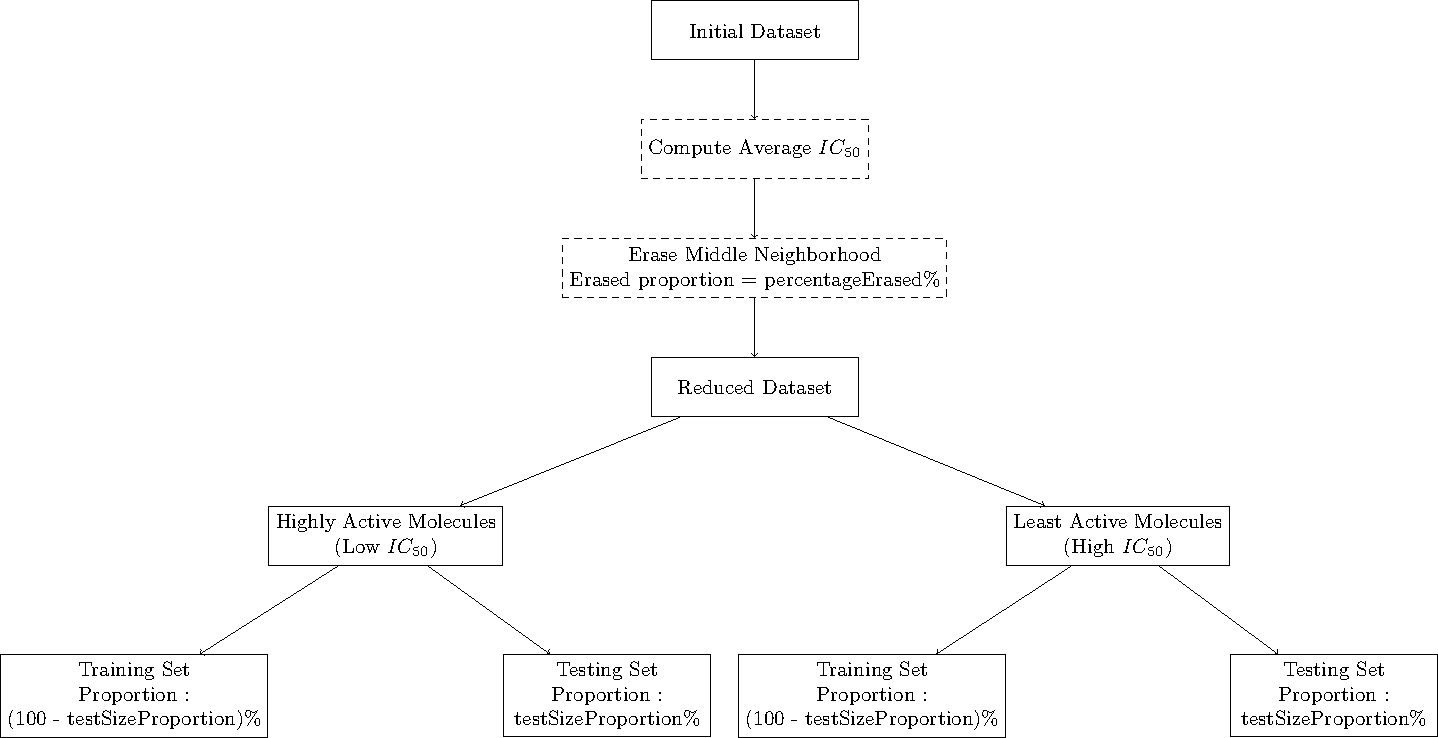
\includegraphics[width = \textwidth]{GeneralSources/DataSplittingDiagram.pdf}
\caption{Scheme of the splitting procedure.}
\label{FigureDataSplittingDiagram}
\end{figure}
\begin{multicols}{2}
Afterward, a Random Forest algorithm is trained using the Sticky Learn \cite{PythonPackageStickitLearn} Python package, which is supported by Microsoft and Google among others. This algorithm generates a large number of random decision trees (determined by the hard-coded variable \emph{numberOfTrees}), which are trained with the training sets. Later, these models are evaluated by predicting the $IC_{50}$ values of the \emph{testing sets}.

Using the results, the \emph{True Positive Rate} (Def. \ref{definitionTruePositiveRate}), \emph{True Negative Rate} (Def. \ref{definitionTrueNegativeRate}), \emph{Classification Accuracy} (Def. \ref{definitionClassificationAccuracy}), and \emph{Matthews Correlation Coefficient} (Def. \ref{definitionMatthewsCorrelationCoeficient}) are computed. Based on these computational results, the variables \emph{percentageErased}, \emph{testSizeProportion}, and \emph{numberOfTrees} are manually adjusted to obtain the best results.

%%%%%%%%%%%%%%%%%%%%%%%%%%%%%%%%%%%%%%%%%%
%%%%%%%%%%%%%%%% BIBLIOGRAPHY %%%%%%%%%%%%%%%%%
%%%%%%%%%%%%%%%%%%%%%%%%%%%%%%%%%%%%%%%%%%


\bibliography{references} 
%%%%%%%%
\section{Abbreviation index}
COX-2 : cyclooxygenase-2\par
AI : Artificial Intelligence\par
ML : Machine Learning\par
RD : Random Forest\par
ID : Identification\par
$IC_{50}$: Half maximal inhibitory concentration \par
$IC_{90}$: 90 percent inhibitory concentration \par
$IC_{99}$: 99 percent inhibitory concentration \par
TP: True Positive\par
FP: False Positive\par
TN: True Negative\par
FN: False Negative
\appendix
\section{Relevant definitions}
\begin{definition}\label{definitionIC50}
$IC_{50}$: Half maximal inhibitory concentration assigned to the drug concentration required for a $50\%$ inhibition a protein. Other quantities such as $IC_{90}$ or $IC_{99}$ are also commonly used. However, $IC_{90}$ is generally approximated as 10 times the $IC_{50}$ concentration in virtue of experimental observations\cite{BookIC50}. For this project, we aim to identify substances with the lowest possible $IC_{50}$, as our goal is to minimize the presence of foreign substances in the living organism.
\end{definition}

\begin{definition}\label{definitionCelecoxib}
Celecoxib: \footnote{UPAC name: 4-[5-(4-Methylphenyl)-3-(trifluoromethyl)pyrazol-1-yl]benzenesulfonamide} drug known to be a selective COX-2 inhibitor (currently is not \emph{highly selective} respect to newer drugs), see Figure (\ref{CelecoxibFigure}). It $IC_{50}$ value is $120$ nM.
\end{definition}

\begin{definition}\label{definitionRofecoxib}
Rofecoxib: \footnote{UPAC name: 4-(4-methylsulfonylphenyl)-3-phenyl-5H-furan-2-one} drug known to be a selective COX-2 inhibitor, see Figure (\ref{RofecoxibFigure}). It $IC_{50}$ value is $180$ nM.
\end{definition}

\begin{figure}[H]
\centering
\scalebox{0.8}{
\chemfig[angle increment=30]{
H_2N-[1]S(=[4]O)(=[-2]O)-[1]*6(-=-(-[1]N*5(-N=(-[-1](-[-4]F)(-[-2]F)-[1])-=(-[4.5]*6(-=-(-[4.5])=-=))-))=-=)
}}
\caption{Chemical graph of Celecoxib.}
\label{CelecoxibFigure}
\end{figure}

\begin{figure}[H]
\centering
\scalebox{0.8}{
\chemfig[angle increment=30]{
-[-1]S(=[-4]O)(=[-2]O)-[1]*6(-=-(-[1]*5(--O-(=[2.25]O)-(-[4.5]*6(-=-=-=))=))=-=)
}}
\caption{Chemical graph of Rofecoxib.}
\label{RofecoxibFigure}
\end{figure}
\begin{definition}\label{definitionPersonCoefficient}
Pearson correlation coefficient: Given set of pairs of data $\{(x_i,y_i)\}_{i=1}^n$ the pearson correlation factor $r_{xy}$ is defined as,
\begin{align}
r_{xy}=\frac{\sum_{i=1}^n(x_i-\bar{x})(y_i-\bar{y})}{\sqrt{\sum_{i=1}^n(x_i-\bar{x}^2)}\sqrt{\sum_{i=1}^n(y_i-\bar{y}^2)}},
\end{align}
where $\bar{x}$ and $\bar{y}$ stand for the average value of ${x_i}_{i=1}^n$ and ${y_i}_{i=1}^n$ respectively. Note that $r_{xy}\in[-1,1]$. Therefore the sign of $r_{xy}$ is tightly related to the sign of alinear regression, more precisely if $x>0$, "$y$" generally\footnote{We would like to remark that the word "generally" stands for "the majority of the cases", since "generally" is commonly interpreted as a non-scientific/non-objective word} increases when "$x$" increases, as well as if $x<0$, "$y$" decreases when "$x$" increases.
\end{definition}
\begin{definition}\label{definitionTruePositiveRate}
True Positive Rate: quantity related to a Machine Learning Model's sensitivity defined as:
\begin{align}
\frac{TP}{TP+FN}
\end{align}
where $TP,FP,TN,FN$ stands for "True Positive", "False Positive", "True Negative" \& "False Negative" respectively.
\end{definition}

\begin{definition}\label{definitionTrueNegativeRate}
True Negative Rate: quantity related to a Machine Learning Model's specificity defined as:
\begin{align}
\frac{TN}{TN+FN}
\end{align}
where $TP,FP,TN,FN$ stands for "True Positive", "False Positive", "True Negative" \& "False Negative" respectively.
\end{definition}

\begin{definition}\label{definitionClassificationAccuracy}
Classification Accuracy: quantity related to a Machine Learning Model's efectiveness defined as:
\begin{align}
\frac{TP+TN}{TP+FP+TN+FN}
\end{align}
where $TP,FP,TN,FN$ stands for "True Positive", "False Positive", "True Negative" \& "False Negative" respectively.
\end{definition}

\begin{definition}\label{definitionMatthewsCorrelationCoeficient}
Matthews Correlation Coefficient: quantity related to a Machine Learning Model's prediction capacity defined as:
{\scriptsize
\begin{align}
\frac{(TP\times TN)-(FP\times FN)}{\sqrt{(TP+FP)\times(TP+FN)\times(TN+FP)\times(TN+FN)}}
\end{align}
}where $TP,FP,TN,FN$ stands for "True Positive", "False Positive", "True Negative" \& "False Negative" respectively.
A Matthews Correlation Coefficient equal to 1 stands for a perfect prediction a Matthews Correlation Coefficient equal to 0 indicates that the classifier’s predictions are no better than random guessing, and a Matthews Correlation Coefficient equal to -1 stand for a total disagreement between predictions and actual outcomes.
\end{definition}

\section{Tables of molecules}
\begin{figure}[H]
\centering
\scalebox{0.8}{
\chemfig[angle increment=30]{
H_2N-S(=[3]O)(=[9]O)-*6(-=-(-N*5(-N=(-R_1)-(-[:45]N=[3]N-[:135]*6(-=-(-R_2)=(-R_3)-=))=-))=-=)
}}
\caption{Template for Celecoxib's azo-derivates with pyrazole as heterocycle.}
\label{figureCelecoxibPyrazole}
\end{figure}

\begin{table}[H]
\centering
\caption{Table of potential photoswitches derivated from Celecoxib's azo-derivates with pyrazole as heterocycle}
\label{tableCelecoxibPyrazole}
\begin{tabular}{c||c|c|c}
Identifier & \ch{R_1} & \ch{R_2} & \ch{R_3} \\\hline\hline
\ref{figureCelecoxibPyrazole}.1 & \ch{CF_3} & \ch{CH_2CH_3}  & \ch{H}\\\hline
\ref{figureCelecoxibPyrazole}.2 & \ch{CF_3} & \ch{CH_2CH_3}  & \ch{F}\\\hline
\ref{figureCelecoxibPyrazole}.3 & \ch{CF_3} & \ch{CH_3}  & \ch{F}\\\hline
\ref{figureCelecoxibPyrazole}.4 & \ch{CF_3} & \ch{OCH_3}  & \ch{H}\\\hline
\ref{figureCelecoxibPyrazole}.5 & \ch{CF_3} & \ch{OCH_3}  & \ch{F}\\\hline
\ref{figureCelecoxibPyrazole}.6 & \ch{CF_3} & \ch{CH_3}  & \ch{H}\\\hline
\ref{figureCelecoxibPyrazole}.7 & \ch{H} & \ch{CH_3}  & \ch{H}\\\hline
\ref{figureCelecoxibPyrazole}.8 & \ch{F} & \ch{CH_3}  & \ch{H}\\\hline
\ref{figureCelecoxibPyrazole}.9 & \ch{Cl} & \ch{CH_3}  & \ch{H}\\\hline
\ref{figureCelecoxibPyrazole}.10 & \ch{Br} & \ch{CH_3}  & \ch{H}\\\hline
\ref{figureCelecoxibPyrazole}.11 & \ch{CH_3} & \ch{CH_3}  & \ch{H}\\\hline
\ref{figureCelecoxibPyrazole}.12 & \ch{H} & \ch{CH_3}  & \ch{F}\\\hline
\ref{figureCelecoxibPyrazole}.13 & \ch{F} & \ch{CH_3}  & \ch{F}\\\hline
\ref{figureCelecoxibPyrazole}.14 & \ch{Cl} & \ch{CH_3}  & \ch{F}\\\hline
\ref{figureCelecoxibPyrazole}.15 & \ch{Br} & \ch{CH_3}  & \ch{F}\\\hline
\ref{figureCelecoxibPyrazole}.16 & \ch{CH_3} & \ch{CH_3}  & \ch{F}
\end{tabular}
\end{table}
\begin{figure}[H]
\centering
\scalebox{0.8}{
\chemname{\chemfig[angle increment=30]{
H_2N-S(=[3]O)(=[9]O)-*6(-=-(-N*5(-N=(-CF_3)-(-[:45]N=[3]N-[:135]*6(-=-(--[3])=N-=))=-))=-=)
}}{Pyridine derivative}}
\par
\vspace{0.5cm}
\scalebox{0.8}{
\chemname{\chemfig[angle increment=30]{
H_3C-S(=[3]O)(=[9]O)-*6(-=-(-N*5(-N=(-CF_3)-(-[:45]N=[3]N-[:135]*6(-=-(-)=N-=))=-))=-=)
}}{\ch{SO_2CH_3} group derivative}}
\caption{Scheme for Celecoxib azo-derivatives based on pyridine and \ch{SO_2CH_3} groups.}
\label{tableCelecoxibPyridine}
\end{figure}

\begin{figure}[H]
\centering
\scalebox{0.8}{
\chemfig[angle increment=30]{
H_2N-S(=[3]O)(=[9]O)-*6(-=-(-*5(-O-(-R_1)=(-[:45]N=[3]N-[:135]*6(-=-(-R_2)=(-)-=))-=))=-=)
}}
\caption{Template for Celecoxib azo-derivatives with furan as a heterocycle.}
\label{figureCelecoxibFuran}
\end{figure}

\begin{table}[H]
\centering
\caption{Table of potential photoswitches derivated from Celecoxib's azo-derivates with furan as heterocycle.}
\label{tableCelecoxibFuran}
\begin{tabular}{c||c|c}
Identifier & \ch{R_1} & \ch{R_2} \\\hline\hline
\ref{figureCelecoxibFuran}.1 & \ch{CF_3} & \ch{H} \\\hline
\ref{figureCelecoxibFuran}.2 & \ch{H} & \ch{H} \\\hline
\ref{figureCelecoxibFuran}.3 & \ch{F} & \ch{H} \\\hline
\ref{figureCelecoxibFuran}.4 & \ch{Cl} & \ch{H} \\\hline
\ref{figureCelecoxibFuran}.5 & \ch{Br} & \ch{H} \\\hline
\ref{figureCelecoxibFuran}.6 & \ch{CH_3} & \ch{H} \\\hline
\ref{figureCelecoxibFuran}.7 & \ch{CF_3} & \ch{F} \\\hline
\ref{figureCelecoxibFuran}.8 & \ch{H} & \ch{F} \\\hline
\ref{figureCelecoxibFuran}.9 & \ch{F} & \ch{F} \\\hline
\ref{figureCelecoxibFuran}.10 & \ch{Cl} & \ch{F} \\\hline
\ref{figureCelecoxibFuran}.11 & \ch{Br} & \ch{F} \\\hline
\ref{figureCelecoxibFuran}.12 & \ch{CH_3} & \ch{F}
\end{tabular}
\end{table}

\begin{figure}[H]
\centering
\scalebox{0.8}{
\chemfig[angle increment=30]{
H_2N-S(=[3]O)(=[9]O)-*6(-=-(-*5(-S-(-R_1)=(-[:45]N=[3]N-[:135]*6(-=-(-R_2)=(-)-=))-=))=-=)
}}
\caption{Template for Celecoxib azo-derivatives with thiophene as a heterocycle.}
\label{figureCelecoxibThiophene}
\end{figure}

\begin{table}[H]
\centering
\caption{Table of potential photoswitches derivated from Celecoxib's azo-derivates with thiophene as heterocycle.}
\label{tableCelecoxibThiophene}
\begin{tabular}{c||c|c}
Identifier & \ch{R_1} & \ch{R_2} \\\hline\hline
\ref{figureCelecoxibThiophene}.1 & \ch{F} & \ch{H} \\\hline
\ref{figureCelecoxibThiophene}.2 & \ch{H} & \ch{F} \\\hline
\ref{figureCelecoxibThiophene}.3 & \ch{Cl} & \ch{F} 
\end{tabular}
\end{table}


\begin{figure}[H]
\centering
\scalebox{0.8}{
\chemfig[angle increment=30]{
H_2N-S(=[3]O)(=[9]O)-*6(-=-(-*5(-\chembelow{N}{H}-(-R_1)=(-[:45]N=[3]N-[:135]*6(-=-(-R_2)=(-R_3)-=))-=))=-=)
}}
\caption{Template for Celecoxib azo-derivatives with pyrrole as a heterocycle.}
\label{figureCelecoxibPyrrole}
\end{figure}

\begin{table}[H]
\centering
\caption{Table of potential photoswitches derivated from Celecoxib's azo-derivates with pyrrole as heterocycle.}
\label{tableCelecoxibPyrrole}
\begin{tabular}{c||c|c|c}
Identifier & \ch{R_1} & \ch{R_2} & \ch{R_3} \\\hline\hline
\ref{figureCelecoxibPyrrole}.1 & \ch{CF_3} & \ch{CH_3} & \ch{H} \\\hline
\ref{figureCelecoxibPyrrole}.2 & \ch{Cl} & \ch{CH_3} & \ch{F} 
\end{tabular}
\end{table}

\begin{figure}[H]
\centering
\scalebox{0.8}{
\chemfig[angle increment=30]{
H_2N-S(=[3]O)(=[9]O)-*6(-=-(-*6(-=(-R_1)-(-N=[2]N-[4]*6(-=-(-R_2)=-=))=-=))=-=)
}}
\caption{Template for Celecoxib azo-derivatives with benzene in place of the original heterocycle.}
\label{figureCelecoxibBenzene}
\end{figure}

\begin{table}[H]
\centering
\caption{Table of potential photoswitches derivated from Celecoxib azo-derivatives with benzene in place of the original heterocycle.}
\label{tableCelecoxibBenzene}
\begin{tabular}{c||c|c}
Identifier & \ch{R_1} & \ch{R_2} \\\hline\hline
\ref{figureCelecoxibBenzene}.1 & \ch{CF_3} & \ch{CH_2CH_3} \\\hline
\ref{figureCelecoxibBenzene}.2 & \ch{CF_3} & \ch{NCH_3COCH_3} \\\hline
\ref{figureCelecoxibBenzene}.3 & \ch{CF_3} & \ch{NHCH_3} \\\hline
\ref{figureCelecoxibBenzene}.4 & \ch{CF_3} & \ch{OCH_3} \\\hline
\ref{figureCelecoxibBenzene}.5 & \ch{Cl} & \ch{CH_3} 
\end{tabular}
\end{table}

\begin{figure}[H]
\centering
\scalebox{0.8}{
\chemfig[angle increment=30]{
H_2N-S(=[3]O)(=[9]O)-*6(-=-(-*5(-\chembelow{N}{H}-*6(-=-(-)=(-[3]N=[4.5]N-[6]*6(-=-(-R_1)=-=))-=)--=))=-=)
}}
\caption{Template for Celecoxib azo-derivatives with indole ring as a heterocycle.}
\label{figureCelecoxibIndole}
\end{figure}


\begin{table}[H]
\centering
\caption{Table of potential photoswitches derivated from Celecoxib azo-derivatives with indole ring as a heterocycle.}
\label{tableCelecoxibIndole}
\begin{tabular}{c||c}
Identifier & \ch{R_1}  \\\hline\hline
\ref{figureCelecoxibIndole}.1 & \ch{H} \\\hline
\ref{figureCelecoxibIndole}.2 & \ch{F} 
\end{tabular}
\end{table}

\begin{figure}[H]
\centering
\scalebox{0.7}{
\chemfig[angle increment=30]{
H_2N-S(=[3]O)(=[9]O)-*6(-=-(-N=[-1.5]N-[-3]*5(=-\chembelow{N}{H}-*6(-=-(-)=(-*6(-=-(-)=-=))-=)--))=-=)
}}
\caption{Template for Celecoxib azo-derivatives with indole ring as a heterocycle.}
\end{figure}

\begin{figure}[H]
\centering
\scalebox{0.7}{
\chemfig[angle increment=30]{
H_2N-S(=[3]O)(=[9]O)-*6(-=-(-N=[-1.5]N-[-3]*5(=-R_1-*5(-R_2-(-)=(-*6(-=-(-R_3)=-=))-=)--))=-=)
}}
\caption{Template for Celecoxib azo-derivatives with two rings of five members joint as a heterocycle.}
\label{figureCelecoxibTwoRings}
\end{figure}

\begin{table}[H]
\centering
\caption{Table of potential photoswitches derivated from Celecoxib azo-derivatives with two rings of five members joint as a heterocycle.}
\label{tableCelecoxibTwoRings}
\begin{tabular}{c||c|c|c}
Identifier & \ch{R_1} & \ch{R_2} & \ch{R_3} \\\hline\hline
\ref{figureCelecoxibTwoRings}.1 & \ch{NH} & \ch{NH} & \ch{H} \\\hline
\ref{figureCelecoxibTwoRings}.2 & \ch{NH} & \ch{O} & \ch{H} \\\hline
\ref{figureCelecoxibTwoRings}.3 & \ch{O} & \ch{NH} & \ch{H} \\\hline
\ref{figureCelecoxibTwoRings}.4 & \ch{O} & \ch{O} & \ch{H} \\\hline
\ref{figureCelecoxibTwoRings}.5 & \ch{NH} & \ch{NH} & \ch{CH_3} \\\hline
\ref{figureCelecoxibTwoRings}.6 & \ch{NH} & \ch{O} & \ch{CH_3} \\\hline
\ref{figureCelecoxibTwoRings}.7 & \ch{O} & \ch{NH} & \ch{CH_3} \\\hline
\ref{figureCelecoxibTwoRings}.8 & \ch{O} & \ch{O} & \ch{CH_3}
\end{tabular}
\end{table}

\end{multicols}
\end{document}